\section{L. Cylinder Results}

\begin{figure}[t]
\centering
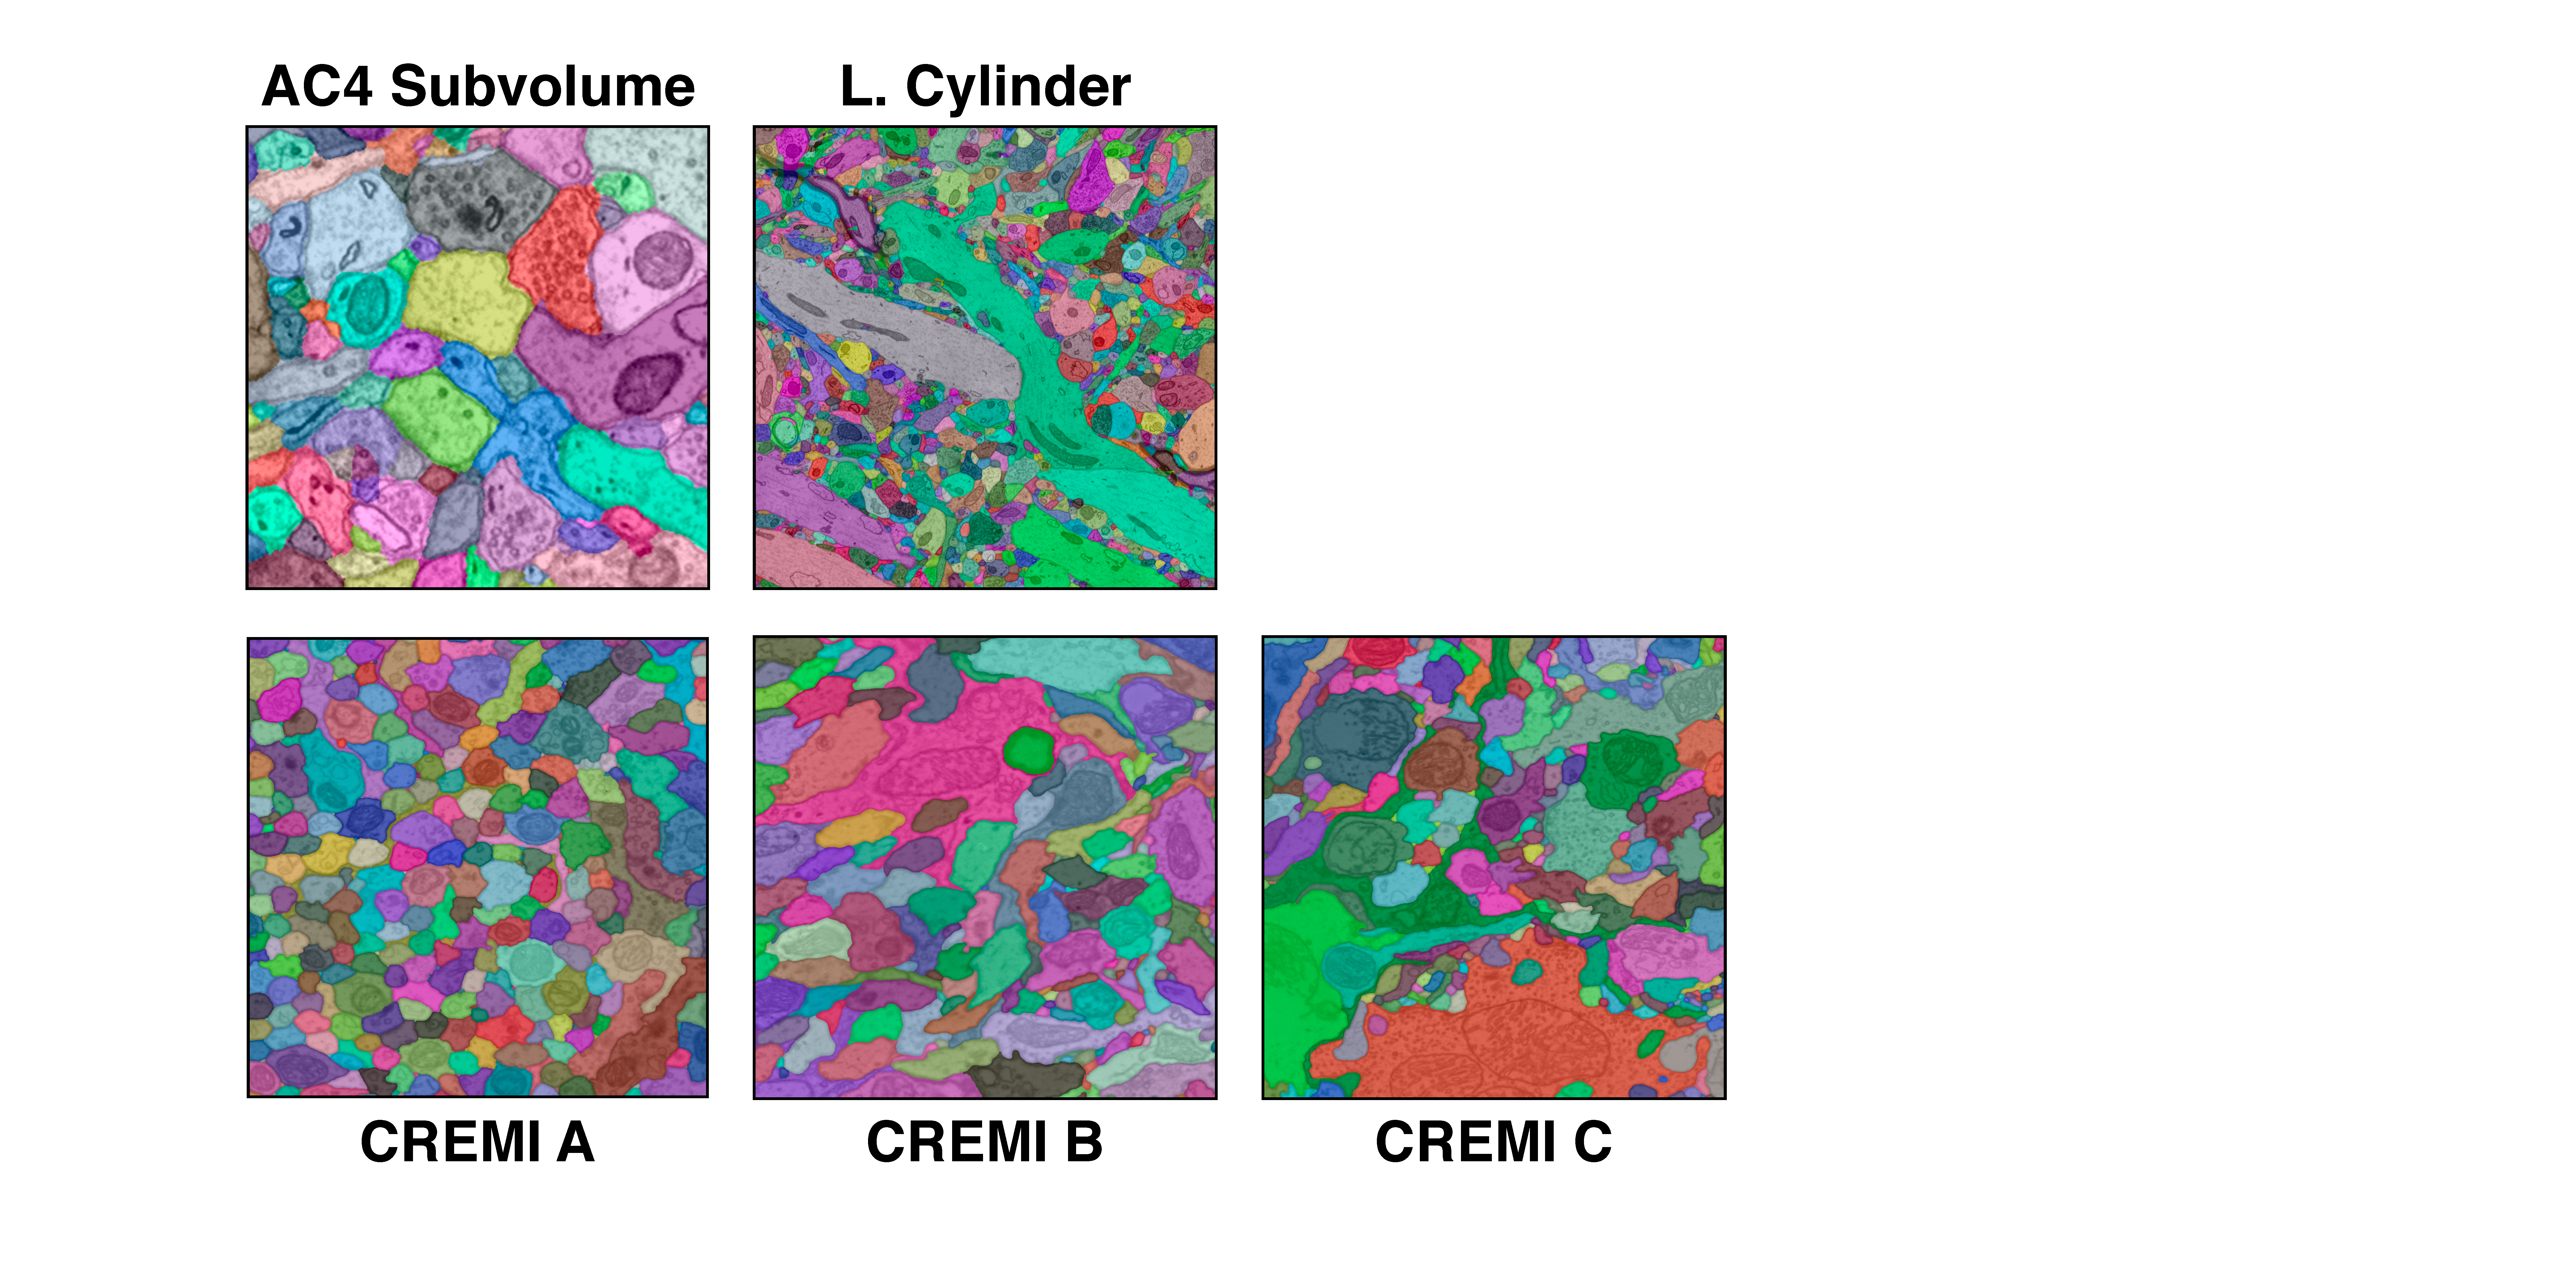
\includegraphics[width=\linewidth]{gfx/datasets.pdf}
\caption{The five different datasets we use for evaluation. The top row shows the first slice of the AC4 and L.~Cylinder mouse brain datasets as reported in the paper. The bottom row shows the first slice of the CREMI A/B/C fruit fly datasets which we used for additional experiments.}
\label{fig:datasets}
\end{figure}

We report experiments and results on the L.~Cylinder dataset in the paper. Figure~\ref{fig:cyltrails} and~\ref{fig:cylboxplot} visualize the reported results measured as variation of information (VI). We compare automatic selection with threshold and selection oracle using focused proofreading and guided proofreading.

\paragraph{Best possible VI.} The selection oracle using guided proofreading does not reach the best possible VI score. We calculate this score by intersecting the initial segmentation and the ground truth. In theory, the classifier should be able to reach this lower bound. However, due to the classification patch size, the membrane probability maps we used included a 30 pixel frame region. Guided proofreading ignores all segments within this frame region, and so cannot reach the best possible VI in some datasets.

\begin{figure}[t]
\centering
\includegraphics[width=\linewidth]{gfx/cyl_trails.pdf}
\caption{Performance comparison of Plaza's focused proofreading and our guided proofreading on the L.~Cylinder dataset as reported in the paper. All measurements are shown as median VI, the lower the better. We compare automatic selection with threshold ($p_t=0.95$, green line) and the selection oracle for accepting or rejecting corrections using each method. Guided proofreading yields better results faster with fewer corrections.}
\label{fig:cyltrails}
\end{figure}

\begin{figure}[t]
\centering
\includegraphics[width=\linewidth]{gfx/cylboxplot.pdf}
\caption{VI distributions of guided proofreading (GP) and focused proofreading (FP) output across slices of the L.~Cylinder dataset, with different error correction approaches. The variation resulting from performance of FP with automatic selection is $7.8\times$ higher than GP (as indicated by the arrow), with median VI of $2.75$ and $SD=0.789$.}
\label{fig:cylboxplot}
\end{figure}


    
    